Considerando as funcionalidades identificadas e documentadas, partiu-se para elaboração de protótipos. Estes protótipos foram construidos considerando as principais funcionalidades a serem desenvolvidas, com o intuito de mostrar à cliente uma representação limitada da solução proposta, mas que permitisse explorar a sua conveniência. O resultado desta prototipação é mostrado a seguir. Embora os protótipos de todas as funcionalidades tenham sido elaborados, apenas os mais relevantes serão mostrados a seguir. Para elaborá-los foi utilizado o software Balsamiq Mockups \cite{Prototipacao:Mockups}.

A tela inicial da aplicação encontra-se ilustrada na Figura  \ref{fig:tela002}. No canto superior direito, há um link para o formulário de autenticação no sistema e também para recuperação de senha, caso algum usuário tenha esquecido da mesma.

\begin{figure}[H]
	\centering
	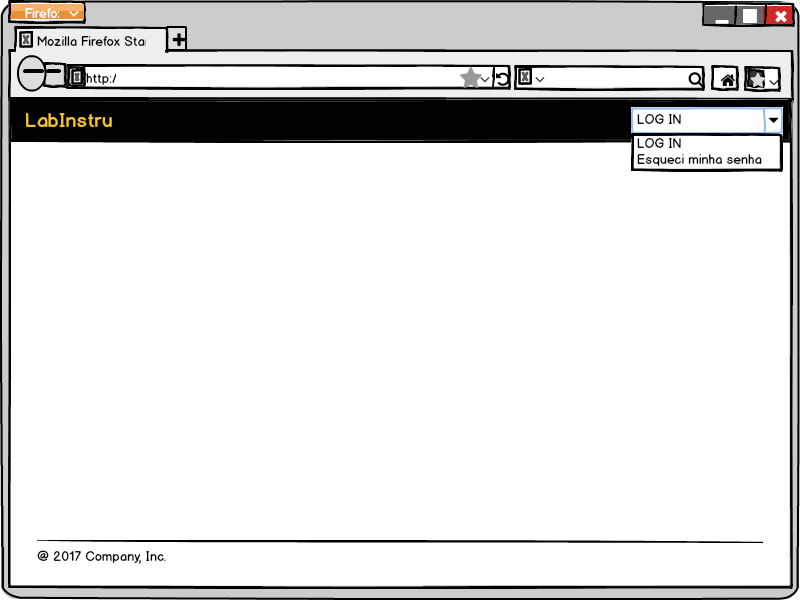
\includegraphics[width=0.65\textwidth]{./img/telas/tela002.png}
	\caption{Tela inicial da aplicação web LabInstru.} \label{fig:tela002}
\end{figure}

Considerando a perspectiva do usuário Administrador, o menu principal da aplicação disponível para o mesmo é mostrado na Figura \ref{fig:tela025}, no qual é possível selecionar a opção ``Cadastrar Usuário'' na aba ``Administração''.  Para efetuar a inclusão de um novo usuário na base de dados, o administrador será redirecionado para o formulário de cadastro ilustrado na Figura \ref{fig:tela027}.


\begin{figure}[H]
	\centering
	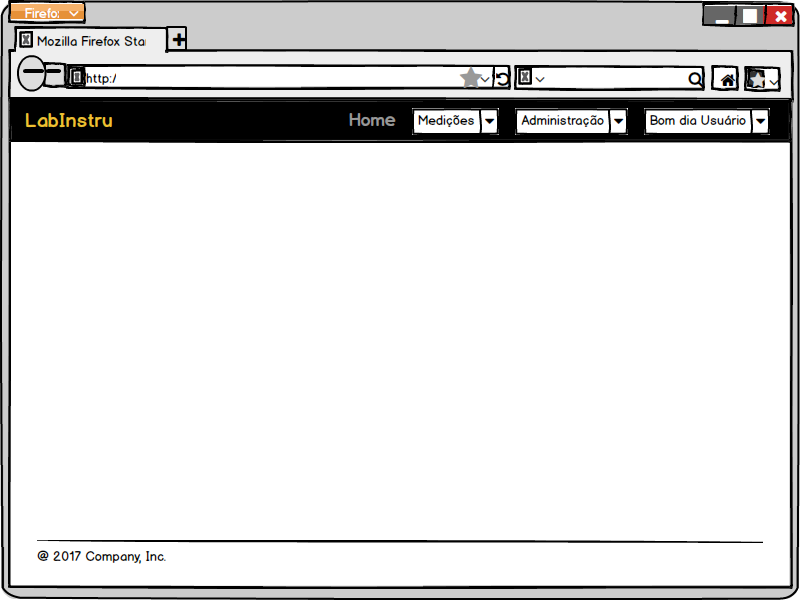
\includegraphics[width=0.65\textwidth]{./img/telas/tela025.png}
	\caption{Protótipo de tela do menu principal da aplicação.} \label{fig:tela025}
\end{figure}


\begin{figure}[H]
	\centering
	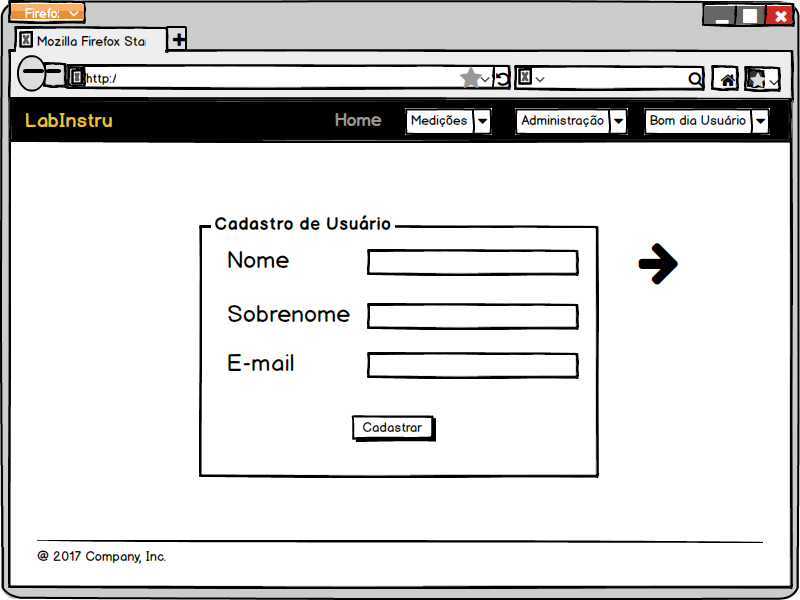
\includegraphics[width=0.65\textwidth]{./img/telas/tela027.png}
	\caption{Protótipo de tela referente ao cadastrado de usuário.} \label{fig:tela027}
\end{figure}

Para exibe uma listagem dos usuários cadastrados na base de dados da aplicação, e posteriormente, caso desejável, fazer a edição ou remoção de um usuário específico, deve-se esoclher a opção ``Listar Usuários'' na aba ``Administração'' do menu principal da aplicação, conforme Figura \ref{fig:tela033}.

\begin{figure}[H]
	\centering
	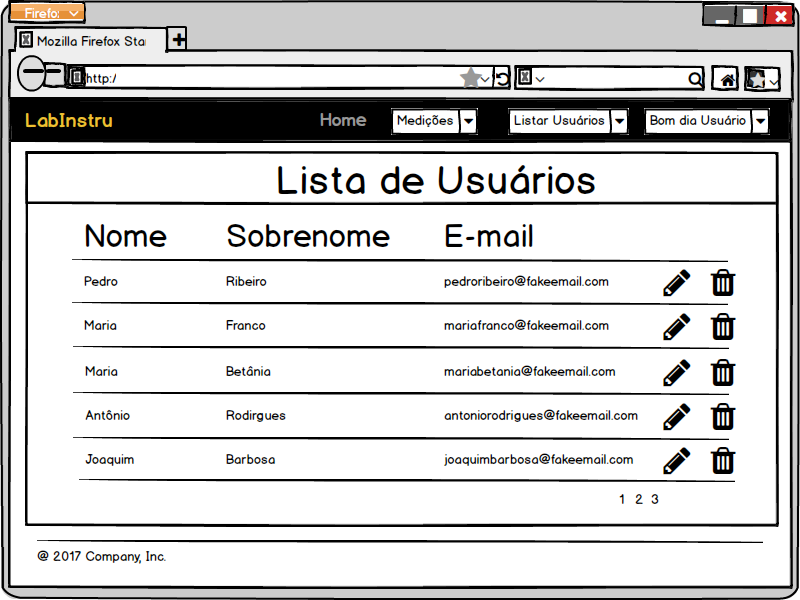
\includegraphics[width=0.65\textwidth]{./img/telas/tela033.png}
	\caption{Protótipo de tela referente à listagem de usuários.} \label{fig:tela033}
\end{figure}

O cadastro de novas medições é efetuado pelo Administrador. Para tanto, este deve utilizar um formulário análogo ao mostrado na Figura \ref{fig:tela053}, em que este deve fornecer um arquivo oriundo da estação meteorológia no formato \texttt{.dat}.

\begin{figure}[H]
	\centering
	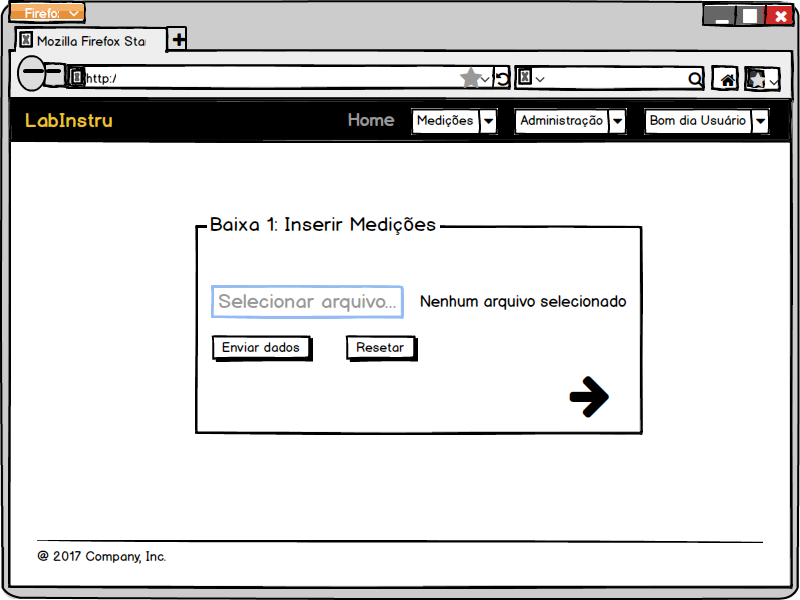
\includegraphics[width=0.65\textwidth]{./img/telas/tela053.png}
	\caption{Protótipo de tela para cadastro de novas medições.} \label{fig:tela053}
\end{figure}

Caso um usuário deseje efetuar uma consulta na base de dados, um formulário detalhado será exibido, conforme ilustrado na Figura  \ref{fig:tela058}, no qual o usuário deve informar os parâmetros para consulta dos dados. Ao submeter a consulta, as respostas serão exibidas conforme ilustrado na Figura \ref{fig:tela062}.

\begin{figure}[H]
	\centering
	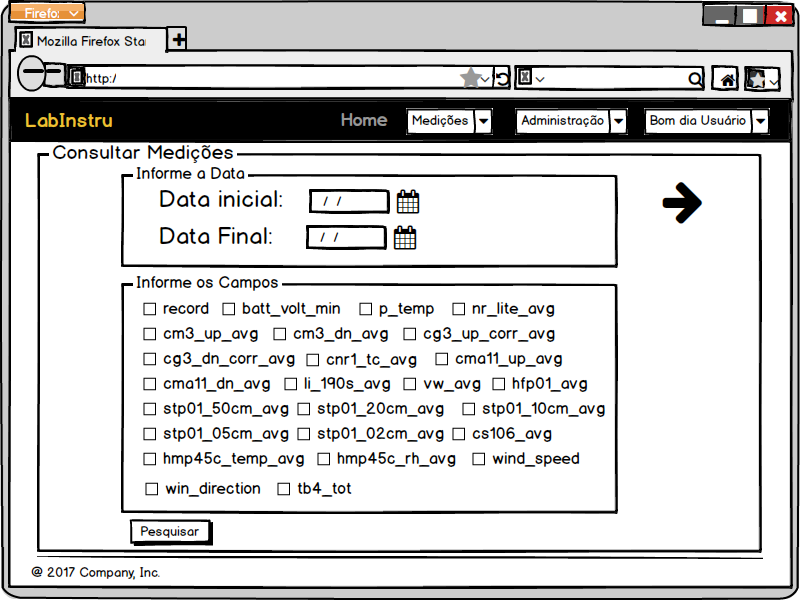
\includegraphics[width=0.65\textwidth]{./img/telas/tela058.png}
	\caption{Protótipo de tela referente ao formulário para consultar medições.} \label{fig:tela058}
\end{figure}

\begin{figure}[H]
	\centering
	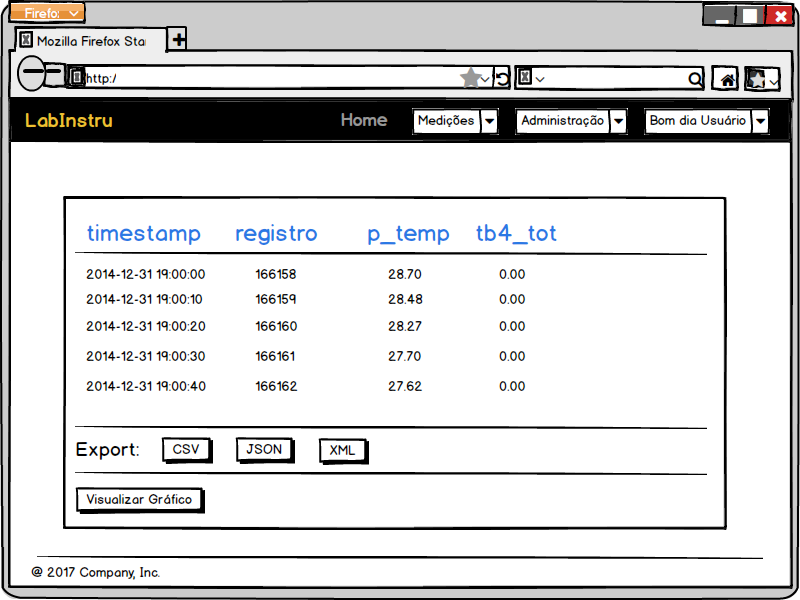
\includegraphics[width=0.65\textwidth]{./img/telas/tela062.png}
	\caption{Protótipo de tela referente à visão de saída a uma consulta de medições.} \label{fig:tela062}
\end{figure}

Por meio do menu principal da aplicação, escolhendo a opção disponibilidade, pertecente à aba de uma determinada estação meteorológica (Baixa 1 ou Baixa 2), vide Figura \ref{fig:tela072}, é possível ter acesso ao calendário de disponibilidade de medições diárias desta estação meteorológica. Esse calendário, conforme ilustrado na Figura \ref{fig:tela073}, tem por objetivo informar quantas medições estão disponíveis em todos os dias do mês escolhido, por meio de cores apropriadas.

\begin{figure}[H]
	\centering
	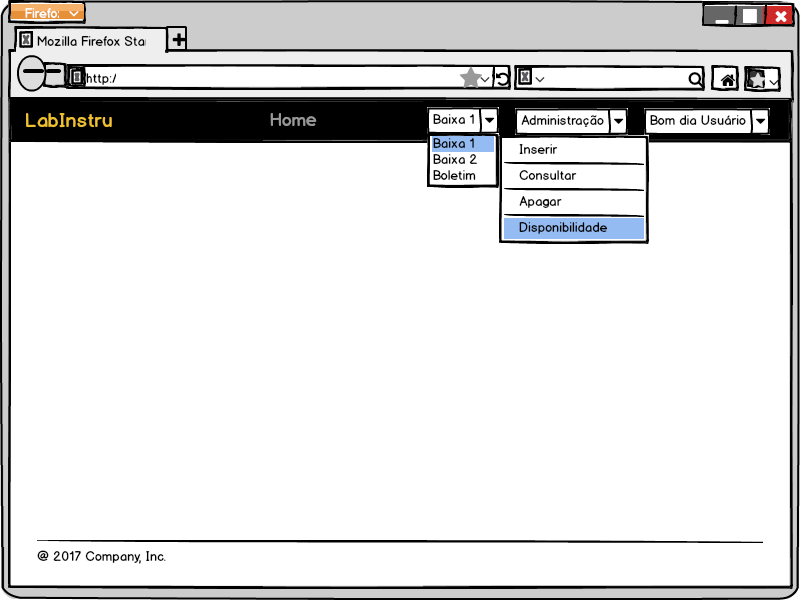
\includegraphics[width=0.65\textwidth]{./img/telas/tela072.png}
	\caption{Navegando no menu para funcionalidade Disponibilidade.} \label{fig:tela072}
\end{figure}

\begin{figure}[H]
	\centering
	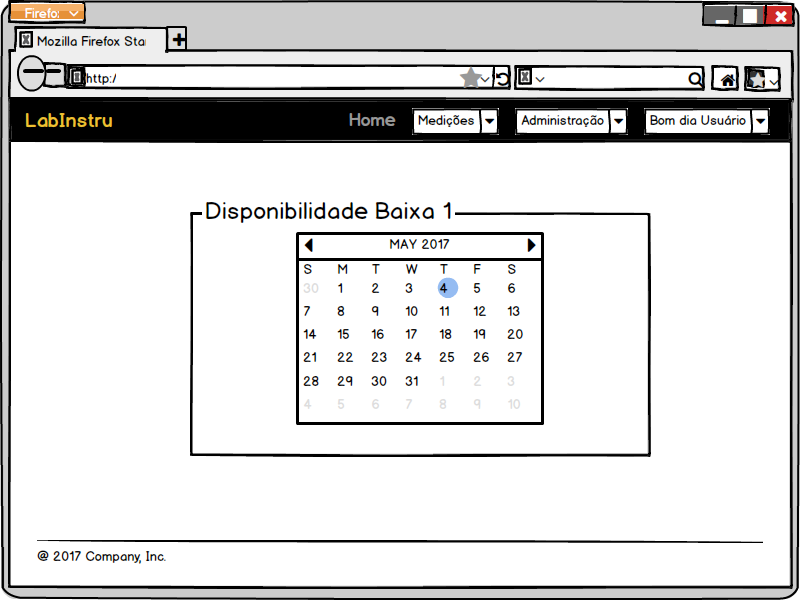
\includegraphics[width=0.65\textwidth]{./img/telas/tela073.png}
	\caption{Tela responsável por exibir o calendário de disponibilidade.} \label{fig:tela073}
\end{figure}

Outra funcionalidade importante na aplicação é o \textit{Boletim Meteorológico}, que pode ser acessado por meio da opção \textit{``Boletim''}, na aba \textit{``Medições''} do menu principal da aplicação. Esse boletim informará diversos dados meteorológicos (temperatura máxima, mínima, índice de calor, etc.) por dia de um determinado mês. A Figura \ref{fig:tela077} ilustra um exemplo de processamento resultante desta funcionalidade.

\begin{figure}[H]
	\centering
	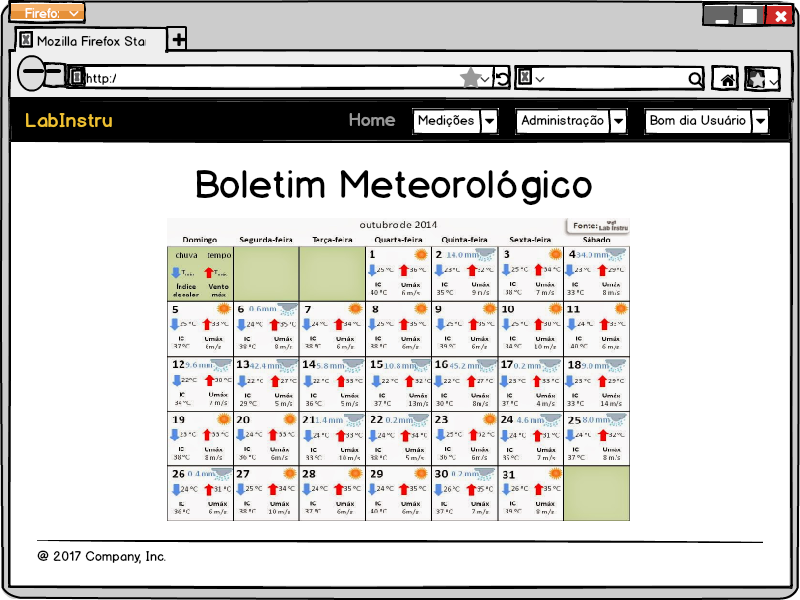
\includegraphics[width=0.65\textwidth]{./img/telas/tela077.png}
	\caption{Protótipo de tela responsável por mostrar o resultado do boletim meteorológico.} \label{fig:tela077}
\end{figure}
